\documentclass[hyperref, UTF8]{ctexart}

\usepackage[a4paper, top=1in, bottom=1.25in, left=1.25in, right=1.25in]{geometry}
\usepackage{float}

\usepackage{xcolor}
\hypersetup{colorlinks=true, linkcolor=black, urlcolor=blue, unicode=true}

% For directory structure
\usepackage{dirtree}

% For show image
\usepackage{graphicx}
\usepackage{caption}
\usepackage{subcaption}

\title{Computer Graphics - HW3}
\author{戴旋\ 13331043}

\begin{document}
	\maketitle
	\tableofcontents

	\section{目录结构}

	\dirtree{%
	.1 / \DTcomment{根目录}.
	.2 doc \DTcomment{项目文档}.
	.3 report.tex.
	.3 report.pdf.
	.2 include \DTcomment{FreeGlut 头文件}.
	.2 lib \DTcomment{FreeGlut静态库}.
	.2 obj \DTcomment{存储中间文件}.
    .2 results \DTcomment{实验结果的截图}.
    .3 rotation.png \DTcomment{自转}.
    .3 revolution.png \DTcomment{公转}.
	.2 src.
	.3 main.cpp \DTcomment{源代码}.
	.2 x64
	.3 freeglut.dll \DTcomment{FreeGlut动态库 x64}.
	.2 freeglut.dll \DTcomment{FreeGlut动态库 x32}.
	.2 main.exe \DTcomment{可执行文件}.
	.2 Makefile \DTcomment{GNU Make}.
	.2 premake5.lua \DTcomment{premake5 脚本}.
	}

	\section{如何运行}
	\begin{enumerate}
		\item Windows\ 或\ Linux \& GNU Make \& GCC
		\begin{itemize}
			\item Windows\ 可直接运行\ main.exe\ (缺少freeglut.dll时,根目录与x64目录下有32位与64位的动态库,可尝试一下)
			\item 在根目录下运行 make 编译生成可执行文件
		\end{itemize}
		\item Mac 或 以上方法无效时,请下载\href{http://premake.github.io/index.html}{premake5},配置好环境变量后,在控制台运行\textbf{premake5 --help}可查看支持的环境。然后在根目录运行\textbf{premake5 xxx}生成相应环境的配置文件。(支持VS,gmake,Xcode)
	\end{enumerate}
	
	\section{程序运行结果}
	\begin{figure}[H]
		\centering
		\begin{subfigure}{0.45\textwidth}
			% pt = px * 72 / DPI
			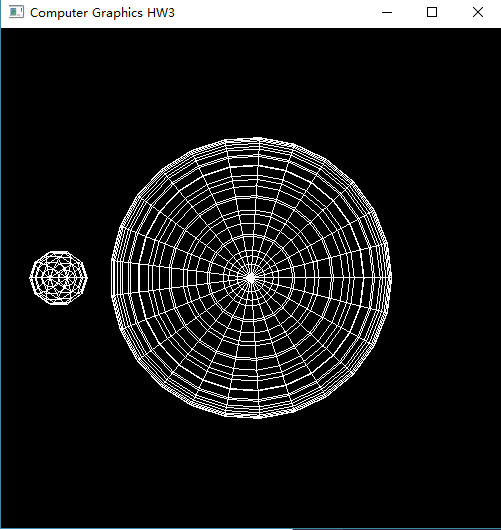
\includegraphics[width=192pt]{../results/rotation.png}
			\caption{自转}
		\end{subfigure}
		~
		\begin{subfigure}{0.45\textwidth}
			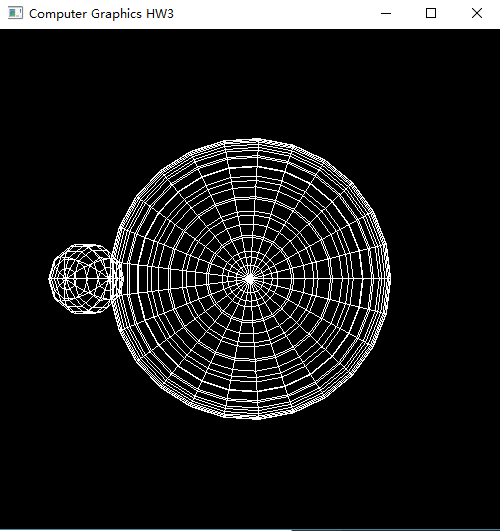
\includegraphics[width=192pt]{../results/revolution.png}
			\caption{公转}
		\end{subfigure}
		\caption{实验结果}
	\end{figure}
\end{document}